\documentclass[12pt,a4paper]{article}

% ---------------------------------------------------------------------------
% PACKAGES
% ---------------------------------------------------------------------------
\usepackage[T1]{fontenc}
\usepackage[utf8]{inputenc}
\usepackage[margin=2.5cm]{geometry}
\usepackage{lmodern}
\usepackage{microtype}
\usepackage{parskip}
\usepackage{booktabs}
\usepackage{amsmath}
\usepackage{tabularx}
\usepackage{graphicx}
\usepackage{float}
\usepackage{xcolor}
\usepackage{hyperref}
\usepackage{tikz}
\usetikzlibrary{positioning, arrows.meta, shapes.geometric, calc, fit}

\setlength{\parskip}{0.75em}
\setlength{\parindent}{0pt}

% Works from the report folder.
\graphicspath{{../docs/img/integration/}} 

\hypersetup{
    colorlinks=true,
    linkcolor=black,
    urlcolor=blue,
    citecolor=black
}

\title{Big Data: Search Engine Project\\Stage 2: Building a Service-Oriented Architecture}
\author{PIE data}
\date{Academic Year 2026/2027}

\begin{document}

\pagenumbering{gobble}

% ---------------------------------------------------------------------------
% COVER
% ---------------------------------------------------------------------------
\begin{titlepage}
    \centering
    \vspace*{1.5cm}

    {\Large Universidad de Las Palmas de Gran Canaria\par}
    \vspace{0.3cm}
    {\large Grado en Ciencia e Ingeniería de Datos\par}

    \vspace{1.5cm}

    {\Huge\bfseries Big Data: Search Engine Project\par}
    \vspace{0.45cm}
    {\LARGE Stage 2: Building a Service-Oriented Architecture\par}

    \vspace{1.6cm}

    \begin{tabular}{ll}
        \textbf{Course:} & Big Data \\
        \textbf{Group:} & PIE data \\
        \textbf{Repository:} & \url{https://github.com/PIE-data/stage_2} \\
    \end{tabular}

    \vspace{1.6cm}

    {\large\bfseries Group members\par}
    \vspace{0.45cm}

    \begin{tabular}{l}
        Marcela Nieto-Kuczyńska \\
        Andrea Patruno \\
        Ivan Colella \\
        Manuel Muñoz Roca \\
    \end{tabular}

    \vfill
    {\large Academic Year 2026/2027\par}
\end{titlepage}

\clearpage
\pagenumbering{roman}
\tableofcontents
\clearpage
\pagenumbering{arabic}

% ---------------------------------------------------------------------------
\section{Introduction and Objectives}
% ---------------------------------------------------------------------------
Stage~2 continues the search engine project by turning the data layer developed in Stage~1 into a
service-oriented system. The storage choices selected in the previous stage are reused, while
Ingestion, Indexing, and Search now run as independent Java processes. The services communicate
through HTTP interfaces and an ActiveMQ message broker, and several replicas of a service can run
on the same Stage~2 host.

The Stage~1 result remains the storage foundation. Downloaded books are stored in the selected
digit-prefix datalake layout, while metadata and the positional inverted index are stored in a
SQLite datamart. The Ingestion Service downloads and splits books, the Indexing Service transforms
them into searchable data, and the Search Service exposes the committed index through a read-only
HTTP API. A Feeder starts ingestion runs and follows their progress, while nginx provides one
front-end entry point for Search replicas.

A main objective of this stage is to keep the pipeline correct when several processes and threads
work at the same time. This requires explicit rules for message delivery, retries, duplicate work,
concurrent file access, SQLite writes, and process failure. The implementation therefore uses
persistent broker messages, transacted JMS consumers, atomic file writes, per-book claims, and
database transactions.

The second objective is to evaluate the behaviour of the complete system under concurrency. The
integration benchmarks vary client concurrency, service threads, batch sizes, and replica counts
for Search, Indexing, and Ingestion. Throughput, latency, queue time, CPU use, and memory use are
measured so that the limits of the single-machine architecture can be identified.

The result of Stage~2 is a complete single-machine search system that can be built, started,
tested, monitored, and stopped as one deployment. Its HTTP interfaces are described by a versioned
OpenAPI specification, its broker messages have a separate event contract, and the complete
pipeline is validated functionally and under load. These results also show which local assumptions
must change in Stage~3, when the architecture moves to several machines.

% ---------------------------------------------------------------------------
\section{System Architecture}
\label{sec:architecture}
% ---------------------------------------------------------------------------
Stage~1 implemented a sequential data pipeline. Stage~2 keeps the same logical order -- download,
split, index, query -- but separates the work into autonomous services. There is no central
controller that calls every stage in order. The pipeline is coordinated mainly by events: a service
reacts to a message, commits its own work, and publishes the event that enables the next stage.

The front-end is deliberately separated from this internal coordination. It sends requests only to
the gateway on port 8080. The gateway forwards them to Search replicas, which read the committed
SQLite datamart. Ingestion and Indexing are never called by the front-end during the normal search
path.

\begin{figure}[H]
	\centering
	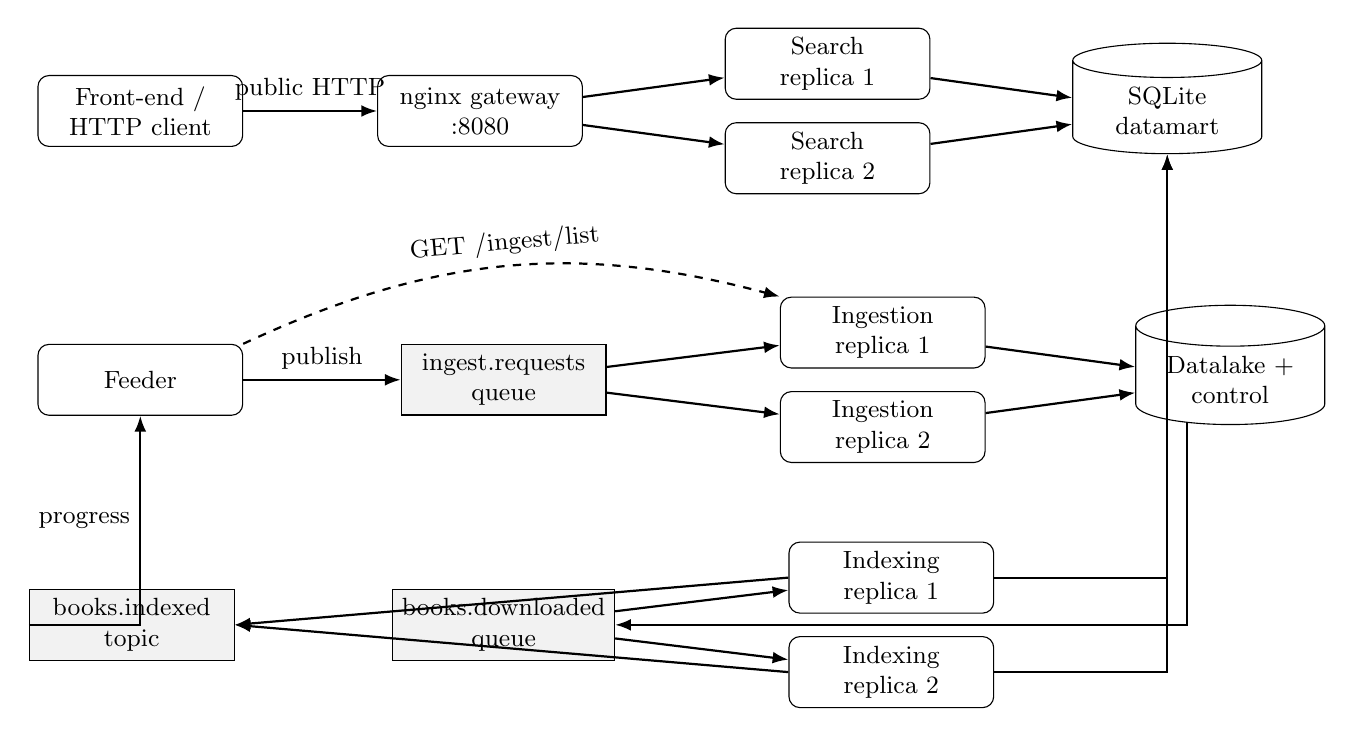
\begin{tikzpicture}[
		node distance=1.3cm and 1.7cm,
		every node/.style={font=\small},
		service/.style={
			draw,
			rounded corners,
			minimum width=2.6cm,
			minimum height=0.9cm,
			align=center
		},
		storage/.style={
			draw,
			cylinder,
			shape border rotate=90,
			aspect=0.28,
			minimum width=2.4cm,
			minimum height=1.2cm,
			align=center
		},
		broker/.style={
			draw,
			rectangle,
			minimum width=2.6cm,
			minimum height=0.8cm,
			align=center,
			fill=gray!10
		},
		arrow/.style={
			-{Latex[length=2mm]},
			thick
		},
		http/.style={
			-{Latex[length=2mm]},
			thick,
			dashed
		}
		]
		
		% Top row: public search path
		\node[service] (client) {Front-end /\\HTTP client};
		
		\node[service, right=of client] (nginx) {nginx gateway\\:8080};
		
		\node[service, right=1.8cm of nginx, yshift=0.6cm] (search1) {Search\\replica 1};
		
		\node[service, right=1.8cm of nginx, yshift=-0.6cm] (search2) {Search\\replica 2};
		
		\node[storage, right=1.8cm of search1, yshift=-0.6cm] (datamart) {SQLite\\datamart};
		
		\draw[arrow] (client) -- node[above]{public HTTP} (nginx);
		\draw[arrow] (nginx) -- (search1);
		\draw[arrow] (nginx) -- (search2);
		\draw[arrow] (search1) -- (datamart);
		\draw[arrow] (search2) -- (datamart);
		
		% Middle row: feeder and ingestion
		\node[service, below=2.5cm of client] (feeder) {Feeder};
		
		\node[broker, right=2.0cm of feeder] (ingestq) {ingest.requests\\queue};
		
		\node[service, right=2.2cm of ingestq, yshift=0.6cm] (ing1) {Ingestion\\replica 1};
		
		\node[service, right=2.2cm of ingestq, yshift=-0.6cm] (ing2) {Ingestion\\replica 2};
		
		\node[storage, right=1.9cm of ing1, yshift=-0.6cm] (datalake) {Datalake +\\control};
		
		\draw[arrow] (feeder) -- node[above]{publish} (ingestq);
		\draw[arrow] (ingestq) -- (ing1);
		\draw[arrow] (ingestq) -- (ing2);
		
		\draw[arrow] (ing1) -- (datalake);
		\draw[arrow] (ing2) -- (datalake);
		
		% Internal HTTP status/list path
		\draw[http]
		(feeder.north east)
		to[bend left=20]
		node[above, sloped]{GET /ingest/list}
		(ing1.north west);
		
		% Bottom row: indexing
		\node[broker, below=2.2cm of ingestq] (downloaded) {books.downloaded\\queue};
		
		\node[service, right=2.2cm of downloaded, yshift=0.6cm] (idx1) {Indexing\\replica 1};
		
		\node[service, right=2.2cm of downloaded, yshift=-0.6cm] (idx2) {Indexing\\replica 2};
		
		\node[broker, left=2.0cm of downloaded] (indexed) {books.indexed\\topic};
		
		\draw[arrow] (datalake.south west) |- (downloaded.east);
		
		\draw[arrow] (downloaded) -- (idx1);
		\draw[arrow] (downloaded) -- (idx2);
		
		\draw[arrow] (idx1.east) -| (datamart.south);
		\draw[arrow] (idx2.east) -| (datamart.south);
		
		\draw[arrow] (idx1.west) -- (indexed.east);
		\draw[arrow] (idx2.west) -- (indexed.east);
		
		\draw[arrow]
		(indexed.west)
		-| node[pos=0.75,left]{progress}
		(feeder.south);
		
	\end{tikzpicture}
	
	\caption{Stage 2 architecture: public Search traffic, broker-driven pipeline,
		replicas, and shared storage.}
	\label{fig:stage2-architecture}
\end{figure}

\subsection{Components and Responsibilities}

\begin{table}[H]
    \centering
    \caption{Processes in the Stage~2 deployment.}
    \label{tab:components}
    \small
    \begin{tabularx}{\textwidth}{p{0.18\textwidth} p{0.12\textwidth} p{0.14\textwidth} X}
        \toprule
        \textbf{Process} & \textbf{Port} & \textbf{Replicas} & \textbf{Responsibility} \\
        \midrule
        Broker & 61616 / 7000 & 1 & Embedded ActiveMQ broker; persistent messages, queues, topic, and monitoring. \\
        Feeder & 7004 & 1 & Chooses books from Stage~1 manifests, skips completed work, publishes ingestion requests, and reports progress. \\
        Ingestion & 7001, 7011, \ldots & 1..N & Downloads and splits books, writes datalake files and receipts, publishes \texttt{books.downloaded}. \\
        Indexing & 7002, 7012, \ldots & 1..N & Parses metadata, builds the positional index, writes the SQLite datamart, publishes \texttt{books.indexed}. \\
        Search & 7003, 7013, \ldots & 1..N & Read-only front-end API over committed data. \\
        Gateway & 8080 & 1 & nginx round-robin entry point in front of Search replicas. \\
        \bottomrule
    \end{tabularx}
\end{table}

All Java services are built as Maven modules and packaged as executable jars. Shared configuration,
HTTP conventions, JSON models, messaging helpers, tokenizer logic, header parsing, and datamart
code live in the \texttt{common} module. Configuration can be provided by defaults, an external
properties file, environment variables, or JVM properties, with later layers overriding earlier
ones.

\subsection{Life of a Book}

The order of the pipeline is encoded by durable state and messages rather than by one orchestration
process. Table~\ref{tab:book-life} shows the state transitions for one book.

\begin{table}[H]
    \centering
    \caption{Life of one book in the Stage~2 pipeline.}
    \label{tab:book-life}
    \small
    \begin{tabularx}{\textwidth}{p{0.08\textwidth} p{0.18\textwidth} X p{0.23\textwidth}}
        \toprule
        \textbf{Step} & \textbf{Owner} & \textbf{Effect} & \textbf{Durable state} \\
        \midrule
        1 & Feeder / HTTP & Publish \texttt{IngestRequested}. & ActiveMQ broker store \\
        2 & Ingestion & Write cleaned header, body, and receipt. & Datalake and \texttt{control/ingestion/} \\
        3 & Ingestion & Publish \texttt{BookDownloaded}. & Broker queue \\
        4 & Indexing & Commit metadata and postings. & \texttt{datamart.db} \\
        5 & Search & New read transactions can see the book. & Same SQLite commit \\
        6 & Indexing & Publish \texttt{BookIndexed} for progress. & Topic notification \\
        \bottomrule
    \end{tabularx}
\end{table}

A book is never announced as downloaded before both datalake files and its receipt are complete.
Likewise, Indexing publishes \texttt{BookIndexed} only after the SQLite commit. Search uses one
read transaction per request, so the result count, ranking data, and returned page come from the
same committed snapshot.

\subsection{Storage and Shared State}

Everything under the default workspace belongs to one machine:

\begin{verbatim}
data/
|-- datalake/<id6[0:2]>/<id6[2:4]>/<id>.header.txt
|-- datalake/<id6[0:2]>/<id6[2:4]>/<id>.body.txt
|-- control/ingestion/hash/<id>.json
|-- control/claims/<id>.lock
|-- control/failed_books.txt
|-- datamarts/datamart.db
`-- broker/
\end{verbatim}

The datalake reuses the Stage~1 digit-prefix layout because Stage~2 always addresses books by id.
The SQLite datamart combines metadata and the positional inverted index in one database so that a
book becomes searchable atomically. ActiveMQ stores unacknowledged messages in KahaDB. These three
stores solve different durability problems but are all local to the same host in Stage~2.

\subsection{Processes, Replicas, and Threads}

A replica is a separate process; a thread is concurrency inside one process. The distinction is
important because the two mechanisms do not protect shared state in the same way.

\begin{table}[H]
    \centering
    \caption{Replication, internal concurrency, and shared-state protection.}
    \label{tab:replicas-threads}
    \small
    \begin{tabularx}{\textwidth}{p{0.16\textwidth} p{0.19\textwidth} p{0.25\textwidth} X}
        \toprule
        \textbf{Service} & \textbf{Replicas} & \textbf{Threads / sessions} & \textbf{Protection of shared state} \\
        \midrule
        Ingestion & Competing consumers & Configurable JMS consumer sessions + HTTP threads & Per-book JVM lock + OS file lock; atomic rename. \\
        Indexing & Competing consumers & Configurable JMS sessions; batches of messages & SQLite \texttt{BEGIN IMMEDIATE}, \texttt{busy\_timeout}; one writer at a time. \\
        Search & nginx upstreams & Jetty request threads & Read-only SQLite connections; no shared writes. \\
        Feeder & Single process & Publisher + HTTP threads & Distinct-id progress set. \\
        Broker & Single process & ActiveMQ internal threads & Persistent KahaDB store. \\
        \bottomrule
    \end{tabularx}
\end{table}

Broker queues distribute work between Ingestion and Indexing replicas with prefetch 1. nginx
distributes HTTP requests between Search replicas. An in-process lock cannot protect two replicas,
so cross-process rules use file locks, SQLite locking, or broker delivery instead.


% ---------------------------------------------------------------------------
\section{API Design and Contracts}
\label{sec:api}
% ---------------------------------------------------------------------------
The HTTP API is documented separately from the broker messages. The implementation distinguishes
the front-end-facing Search API from internal and operational endpoints. The complete HTTP
contract is versioned in \texttt{api/openapi.yaml}, while \path{docs/API_INVENTORY.md} records
the provider, consumer, and purpose of every route.

\subsection{Front-End-Facing API}

The front-end communicates with Search through the nginx gateway on port 8080. It does not read
local files, access SQLite directly, or interact with the message broker.

\begin{table}[H]
    \centering
    \caption{Front-end-facing Search endpoints.}
    \small
    \begin{tabularx}{\textwidth}{p{0.22\textwidth} p{0.20\textwidth} X}
        \toprule
        \textbf{Route} & \textbf{Provider / consumer} & \textbf{Purpose} \\
        \midrule
        \texttt{GET /search} & Search / front-end & Keyword search with optional author, language, and release-year filters plus pagination. \\
        \texttt{GET /search/filters} & Search / front-end & Return the languages and release-year range available in the current datamart. \\
        \texttt{GET /books/\{book\_id\}} & Search / front-end & Return metadata for one indexed book. \\
        \bottomrule
    \end{tabularx}
\end{table}

The required query parameter is \texttt{q}. Optional filters are \texttt{author},
\texttt{language}, and \texttt{year}; pagination uses \texttt{offset} and \texttt{limit}.
Multiple normalized query terms use AND semantics. Results are ranked with TF-IDF and then by book
id. Invalid parameters return a documented HTTP 400 error, while a valid query with no matches
returns HTTP 200 with an empty result list.

\subsection{Internal and Operational APIs}

Internal and operational routes are used by the Feeder, scripts, monitoring, and validation rather
than by the front-end.

\begin{table}[H]
    \centering
    \caption{Main internal and operational endpoints.}
    \scriptsize
    \begin{tabularx}{\textwidth}{p{0.26\textwidth} p{0.20\textwidth} X}
        \toprule
        \textbf{Route} & \textbf{Provider / consumer} & \textbf{Purpose} \\
        \midrule
        \texttt{POST /ingest/\{book\_id\}} & Ingestion / operator, checks & Accept one ingestion request. \\
        \texttt{GET /ingest/status/\{book\_id\}} & Ingestion / scripts, checks & Report downloaded, failed, or not found. \\
        \texttt{GET /ingest/list} & Ingestion / Feeder & Return completed ingestion ids so the Feeder can skip them. \\
        \texttt{POST /index/update/\{book\_id\}} & Indexing / operator, checks & Index or re-index one completed book. \\
        \texttt{POST /index/rebuild} & Indexing / operator, checks & Rebuild the complete datamart. \\
        \texttt{GET /index/status} & Indexing / monitoring & Return index counts and state. \\
        \texttt{POST /feeder/run} & Feeder / operator, benchmarks & Start a run from a manifest. \\
        \texttt{GET /feeder/status} & Feeder / monitoring & Report requested and indexed progress. \\
        \texttt{GET /broker/stats} & Broker / monitoring, benchmarks & Return queue depth and timing statistics. \\
        \texttt{GET /status} & Every service / scripts & Standard health endpoint. \\
        \bottomrule
    \end{tabularx}
\end{table}

\subsection{Non-HTTP Coordination Contract}

Most pipeline coordination does not use HTTP. It is defined in \texttt{docs/EVENTS.md} and carried
by ActiveMQ.

\begin{table}[H]
    \centering
    \caption{Broker destinations used by the pipeline.}
    \small
    \begin{tabularx}{\textwidth}{p{0.22\textwidth} p{0.12\textwidth} p{0.20\textwidth} X}
        \toprule
        \textbf{Destination} & \textbf{Type} & \textbf{Producer} & \textbf{Meaning / consumer} \\
        \midrule
        \texttt{ingest.requests} & Queue & Feeder / Ingestion HTTP & Request one book; consumed by one Ingestion replica. \\
        \texttt{books.downloaded} & Queue & Ingestion & Book files and receipt are complete; consumed by one Indexing replica. \\
        \texttt{books.indexed} & Topic & Indexing & Book is committed and searchable; used for Feeder progress and monitoring. \\
        \texttt{ActiveMQ.DLQ} & Queue & Broker & Messages that still fail after the configured redeliveries. \\
        \bottomrule
    \end{tabularx}
\end{table}

\subsection{Completion Semantics and Errors}

A new \texttt{POST /ingest/\{book\_id\}} returns HTTP 202 after the request is published to
ActiveMQ; this does not mean that the book has already been downloaded or indexed. If the book is
already ingested, the endpoint returns HTTP 200. Indexing HTTP operations return HTTP 200 only
after the datamart operation has completed.

The specification also records validation and error behaviour. Examples include HTTP 400 for
invalid parameters, HTTP 404 for unknown resources, HTTP 409 for conflicting Indexing states, and
HTTP 503 when an operation depends on an unavailable broker or busy datamart. Error responses use
a common JSON shape with an error code and message.

\subsection{Specification and Validation Evidence}

The API work is delivered in four parts:
\begin{itemize}
    \item \texttt{api/openapi.yaml}: the versioned HTTP contract, including parameters, schemas,
    defaults, status codes, examples, pagination, ordering, filtering, and completion semantics;
    \item \path{docs/API_INVENTORY.md}: the endpoint inventory with provider, consumer, and purpose;
    \item \texttt{api/api-checks.http}: runnable manual HTTP requests;
    \item \texttt{scripts/check-api.sh}: automated checks of the running deployment, including the
    event checks defined for broker coordination.
\end{itemize}

The final validation was run against the full deployment and returned \textbf{32 PASS, 0 FAIL, 0
SKIP}. This provides evidence that the running endpoints and the documented contract agree for the
validated cases.


% ---------------------------------------------------------------------------
\section{Microservice Implementation}
\label{sec:implementation}
% ---------------------------------------------------------------------------
The services are implemented in Java and built as a Maven multi-module project. The project uses
Java~17 as the compilation target, Javalin~6.1.3 for HTTP services, Gson~2.11.0 for JSON handling,
ActiveMQ Classic for broker coordination, and SQLite for the searchable datamart. Shared code is
kept in the \texttt{common} module so that services use the same configuration, data models,
tokenizer rules, event formats, and datamart code.

\subsection{Ingestion Service}

Ingestion receives a book id either from the \texttt{ingest.requests} queue or from its HTTP API.
It downloads the Project Gutenberg text, finds the expected start and end markers, separates the
header and body, cleans the text according to the Stage~1 specification, and writes the selected
datalake layout.

Writes use a temporary \texttt{.part} file followed by an atomic move to the final path. A receipt
marks a completely ingested book. To avoid two replicas processing the same book at the same time,
Ingestion combines an in-process lock with an OS file lock on a per-book claim. Repeated requests
are safe because an existing receipt is detected before new work is performed. The 20 golden books
are used to verify compatibility with Stage~1.

\subsection{Indexing Service}

Indexing consumes \texttt{BookDownloaded} events and can also be called through administrative
HTTP routes. It reads the completed header and body, parses metadata, tokenizes the text, builds the
positional inverted index, and writes metadata, terms, and postings into
\texttt{data/datamarts/datamart.db}.

SQLite uses WAL mode. Indexing is the logical writer and Search is read-only. Re-indexing replaces
the existing rows for a book instead of creating duplicates. Broker messages can be processed in
batches; the default batch size is 20 with a 200~ms batch wait. The canonical export for the golden
dataset is checked against the Stage~1 SHA-256 oracle.

\subsection{Search Service}

Search exposes the front-end HTTP API and never modifies the datamart. Each request uses a
read-only SQLite connection and one read transaction. Query terms are normalized with the Stage~1
tokenizer. Multiple terms use AND semantics, and the optional filters are author, language, and
Gutenberg release year.

Ranking uses TF-IDF:
\[
    \operatorname{score}(d)=\sum_{t \in q} tf(t,d)\,\ln\!\left(\frac{N}{df(t)}\right).
\]
Results are ordered by decreasing score and then increasing book id. Search can run as several
replicas on different ports, with nginx providing one public gateway.

\subsection{Broker and Feeder}

The broker runs as its own Java process with persistent KahaDB storage. It provides the two work
queues, the indexed topic, and the Dead Letter Queue. Consumers use transacted JMS sessions, and
the failover transport reconnects clients after a broker restart.

The Feeder starts pipeline work from the Stage~1 corpus manifests. Before publishing new requests,
it checks the completed ingestion ids and skips books that are already present. It listens to
\texttt{books.indexed} to report progress through \texttt{/feeder/status}.

\subsection{Readiness and Failure Handling}

Every HTTP service exposes \texttt{GET /status}. The deployment scripts start services in order and
wait for their readiness endpoints before continuing. A crashed service is not automatically
restarted by the process manager; unacknowledged broker work can instead be redelivered to a
remaining consumer replica.

Transient consumer failures cause the JMS transaction to roll back and the message to be
redelivered. Permanent ingestion failures such as a missing Gutenberg book are recorded and
completed without repeated retries. Malformed messages that still fail after the configured
redeliveries end in \texttt{ActiveMQ.DLQ}.


% ---------------------------------------------------------------------------
\section{Design Decisions}
\label{sec:design}
% ---------------------------------------------------------------------------
\subsection{Reuse of Stage 1 Contracts and Oracles}

Stage~2 changes the execution architecture without intentionally changing the meaning of the data.
The Java tokenizer is checked against the frozen Stage~1 token oracle, the metadata parser against
the golden metadata records, and the datamart writer against the same canonical SHA-256 export.
This gives a correctness reference while the implementation moves from one pipeline to independent
services.

\subsection{Choreography Instead of a Central Control Module}

The project uses choreography with ActiveMQ rather than a central orchestrator. Each service owns
one responsibility and reacts to events. The Feeder publishes an ingestion request, Ingestion
publishes \texttt{BookDownloaded} when the files are complete, and Indexing publishes
\texttt{BookIndexed} after the database commit.

This choice lets replicas become competing consumers without changing the workflow logic. It also
buffers temporary differences in service speed: if Ingestion is faster than Indexing, completed
books wait in \texttt{books.downloaded} rather than blocking the Ingestion process.

\subsection{At-Least-Once Delivery and Idempotency}

The messaging model is at least once, so duplicate delivery is possible. The project therefore
makes consumers idempotent instead of assuming exactly-once delivery. Ingestion skips a book with
an existing receipt, Indexing replaces the previous rows for the same book, and the Feeder counts
distinct ids.

Broker consumers use transacted JMS sessions. The general sequence is:
\begin{verbatim}
receive -> do work -> commit storage
-> send next event -> session.commit()
\end{verbatim}
If the transaction is not committed, the input message can be redelivered. The redelivery policy
uses up to five redeliveries with delays of 1, 2, 4, 8, and 16 seconds before a repeatedly failing
message reaches the DLQ.

\subsection{Local Storage and SQLite}

The Stage~1 datalake layout is kept because Stage~2 reads books by id. SQLite is kept for the
searchable datamart because it provides transactions, a simple single-file deployment, and WAL
mode for concurrent readers. The important limitation is that the database has one writer at a
time. This is acceptable for Stage~2 but becomes a measured bottleneck when several Indexing
replicas share the same file.

Atomic file writes and per-book claims protect Ingestion on the same host. These mechanisms depend
on one local filesystem and one kernel, so they are assumptions that must change for Stage~3.

\subsection{Replicas, Threads, and Single-Machine Deployment}

Replicas and threads are treated as different forms of concurrency. Replicas are separate service
processes; threads or JMS sessions add concurrency inside one process. On the Stage~2 host they all
share the same physical resources, so adding workers may increase contention rather than
throughput.

nginx is used as a round-robin gateway for Search replicas. The deployment scripts keep ports,
replica counts, data paths, thread settings, JVM heap, and Indexing batch settings in one
configuration so that the complete single-machine setup can be reproduced.

\subsection{Functional Validation Before Benchmarking}

A 20-book full-pipeline smoke test completed all 20 books, retrieved every id through the gateway,
drained both work queues, and left the DLQ empty. A second test requested 100 books with two
replicas of Ingestion, Indexing, and Search. One Indexing replica was killed after 70 books had
been observed as indexed; the remaining replica completed all 100 books and the final queues were
empty. These tests show that the event and replica design continues processing after a replica is
lost.

% ---------------------------------------------------------------------------
\section{Benchmarks and Results}
\label{sec:benchmarks}
% ---------------------------------------------------------------------------
\subsection{Dataset, Method, and Measures}

The integration benchmark uses the delivered Stage~2 code and a tier-1000 workspace. Every
configuration is repeated three times and reported as mean $\pm$ standard deviation unless stated
otherwise. The client, broker, services, and monitor all run on the same WSL machine. Before a run,
state that could affect the experiment is reset; runs are rejected if a book is lost, an error is
reported, a pipeline book is skipped as already ingested, or a message reaches the DLQ.

\begin{table}[H]
    \centering
    \caption{Integration benchmark environment and baseline.}
    \label{tab:benchmark-setup}
    \small
    \begin{tabularx}{\textwidth}{p{0.22\textwidth} X}
        \toprule
        \textbf{Item} & \textbf{Value} \\
        \midrule
        Host & Intel Core i7-1255U laptop, 12 logical CPUs visible to WSL, Windows + WSL~2 Ubuntu, 10~GiB WSL RAM. \\
        Runtime & OpenJDK 21.0.12, code compiled for Java~17; nginx 1.28.3; 64--512~MiB JVM heap. \\
        Code & Benchmark commit \texttt{19e2b1b}, 4 November 2026. \\
        Data & 1,000 Gutenberg books; 1,000-book datamart with 366,187 distinct terms. \\
        Search workload & 300 fixed queries from three document-frequency groups; 70\% one term, 30\% two terms; 22.7\% empty answers. \\
        Baseline & One replica per service; Indexing two consumer sessions, batch 20, 200~ms batch wait; HTTP threads 8--64; one nginx worker. \\
        Search runs & Closed loop; 10~s warm-up; 60~s measured (X1 uses 5~s + 30~s). \\
        Indexing runs & I1--I3 send 1,000 messages at once; I4 sends 200 books at controlled rates. \\
        \bottomrule
    \end{tabularx}
\end{table}

The main questions are whether Search scales with client concurrency and replicas, whether Indexing
benefits from larger batches, more consumer sessions, or more replicas, whether Ingestion replicas
increase end-to-end throughput, and how much Search and Indexing interfere when they share one
machine.

\subsection{Search Concurrency}

\begin{table}[H]
    \centering
    \caption{S1: one Search replica, direct port, increasing client concurrency.}
    \label{tab:s1}
    \small
    \begin{tabular}{rrrrr}
        \toprule
        \textbf{Clients} & \textbf{Queries/s} & \textbf{Mean ms} & \textbf{p95 ms} & \textbf{p99 ms} \\
        \midrule
        1  & $1017 \pm 4$   & $0.98 \pm 0.01$ & $1.74 \pm 0.04$ & $2.37 \pm 0.07$ \\
        2  & $1829 \pm 55$  & $1.09 \pm 0.04$ & $2.09 \pm 0.05$ & $2.61 \pm 0.14$ \\
        4  & $3037 \pm 149$ & $1.31 \pm 0.07$ & $2.38 \pm 0.09$ & $3.09 \pm 0.15$ \\
        8  & $4373 \pm 674$ & $1.86 \pm 0.31$ & $3.66 \pm 0.90$ & $6.27 \pm 3.00$ \\
        16 & $6101 \pm 177$ & $2.62 \pm 0.08$ & $5.21 \pm 0.20$ & $7.88 \pm 0.66$ \\
        32 & $7875 \pm 208$ & $4.06 \pm 0.11$ & $8.64 \pm 0.26$ & $12.69 \pm 0.43$ \\
        \bottomrule
    \end{tabular}
\end{table}

\begin{figure}[H]
    \centering
    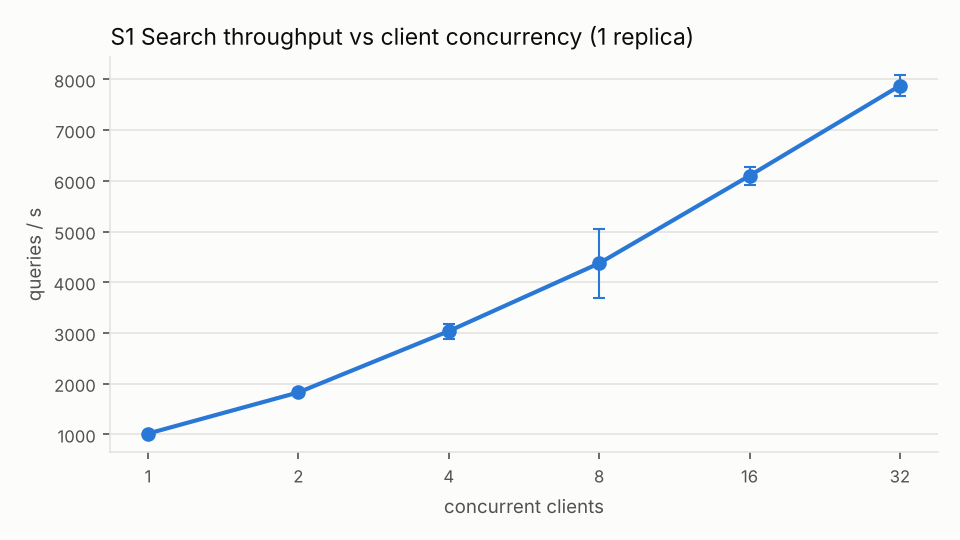
\includegraphics[width=0.78\textwidth]{s1-throughput.png}
    \caption{Search throughput as client concurrency increases. Error bars show one standard deviation.}
    \label{fig:s1-throughput}
\end{figure}

\begin{figure}[H]
    \centering
    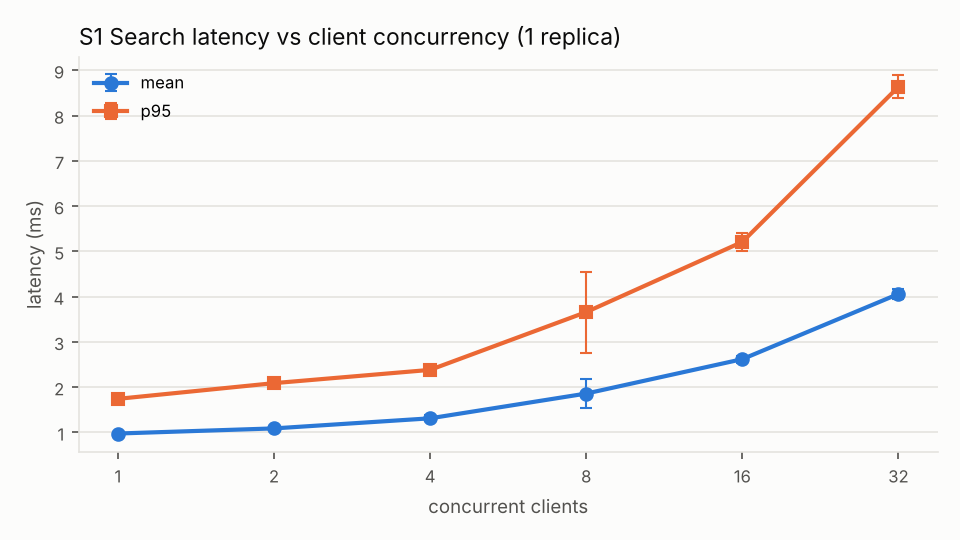
\includegraphics[width=0.78\textwidth]{s1-latency.png}
    \caption{Search p95 latency as client concurrency increases.}
    \label{fig:s1-latency}
\end{figure}

Throughput grows almost linearly only at the beginning. From 16 to 32 clients the number of clients
doubles, but throughput grows by 29\% while p95 latency grows by 66\%. At 32 clients the Search
process uses about seven logical CPUs at p90 and the WSL host is already heavily loaded. Search has
no writer lock in this experiment, so the observed saturation is a CPU limit rather than a database
serialization limit.

\subsection{Search Replicas and Gateway Cost}

\begin{table}[H]
    \centering
    \caption{S2: Search replicas behind nginx.}
    \label{tab:s2}
    \small
    \begin{tabular}{rrrrr}
        \toprule
        \textbf{Replicas} & \textbf{16 clients q/s} & \textbf{p95 ms} & \textbf{32 clients q/s} & \textbf{p95 ms} \\
        \midrule
        1 & $4353 \pm 44$ & $6.10 \pm 0.10$ & $5147 \pm 102$ & $10.54 \pm 0.37$ \\
        2 & $4019 \pm 38$ & $6.74 \pm 0.08$ & $4428 \pm 192$ & $12.86 \pm 0.99$ \\
        3 & $3647 \pm 75$ & $7.78 \pm 0.28$ & $4074 \pm 125$ & $14.46 \pm 1.18$ \\
        \bottomrule
    \end{tabular}
\end{table}

\begin{figure}[H]
    \centering
    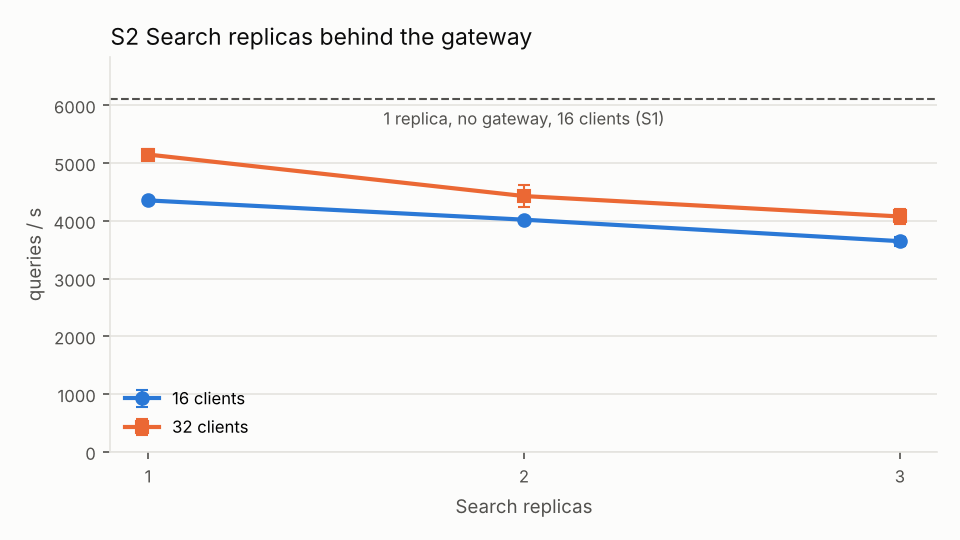
\includegraphics[width=0.78\textwidth]{s2-replicas.png}
    \caption{Search throughput behind nginx as replicas are added.}
    \label{fig:s2-replicas}
\end{figure}

The gateway has a measurable cost on one host. With one replica and 16 clients, throughput drops
from 6101 q/s on the direct port to 4353 q/s through nginx. More Search replicas reduce throughput
further. The replicas share the same cores, so the additional JVMs, context switches, and per-process
caches add work without adding CPU capacity. Replication is still useful for availability -- the
failure tests show that -- but it is not a speedup mechanism on this machine.

\subsection{Indexing: Batch Size, Sessions, and Replicas}

\begin{table}[H]
    \centering
    \caption{I1--I3: Indexing throughput at saturation.}
    \label{tab:indexing-saturation}
    \small
    \begin{tabularx}{\textwidth}{p{0.22\textwidth} p{0.31\textwidth} X}
        \toprule
        \textbf{Experiment} & \textbf{Configurations} & \textbf{Throughput (books/s)} \\
        \midrule
        I1 batch size & 1 / 5 / 20 / 50 & $6.08 \pm 0.28$ / $11.23 \pm 0.29$ / $18.37 \pm 0.27$ / $22.30 \pm 0.11$ \\
        I2 consumer sessions & 1 / 2 / 4 & $17.69 \pm 1.00$ / $18.39 \pm 0.53$ / $16.19 \pm 1.61$ \\
        I3 replicas & 1 / 2 / 3 & $17.92 \pm 0.68$ / $14.51 \pm 3.19$ / $10.10 \pm 1.55$ \\
        \bottomrule
    \end{tabularx}
\end{table}

\begin{figure}[H]
    \centering
    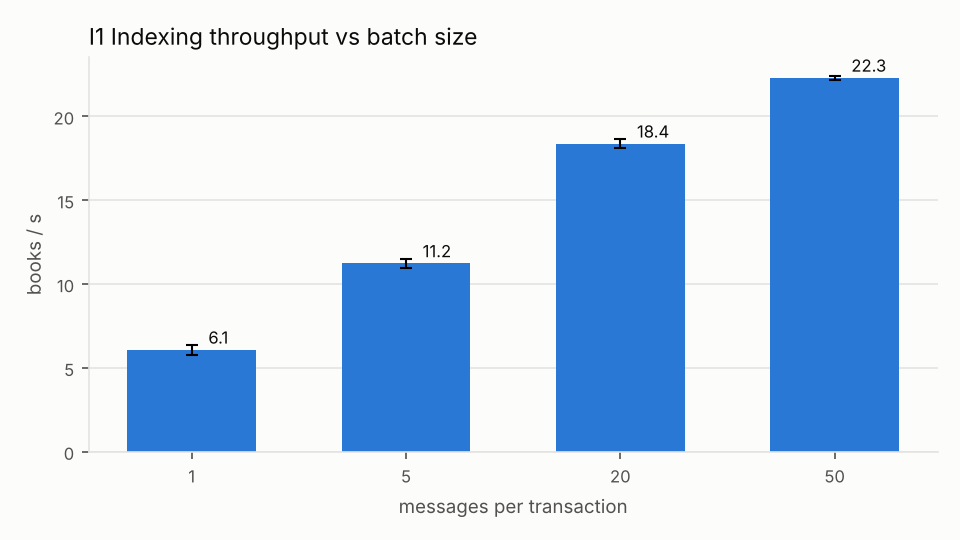
\includegraphics[width=0.75\textwidth]{i1-batch.png}
    \caption{Indexing throughput versus transaction batch size.}
    \label{fig:i1}
\end{figure}

\begin{figure}[H]
    \centering
    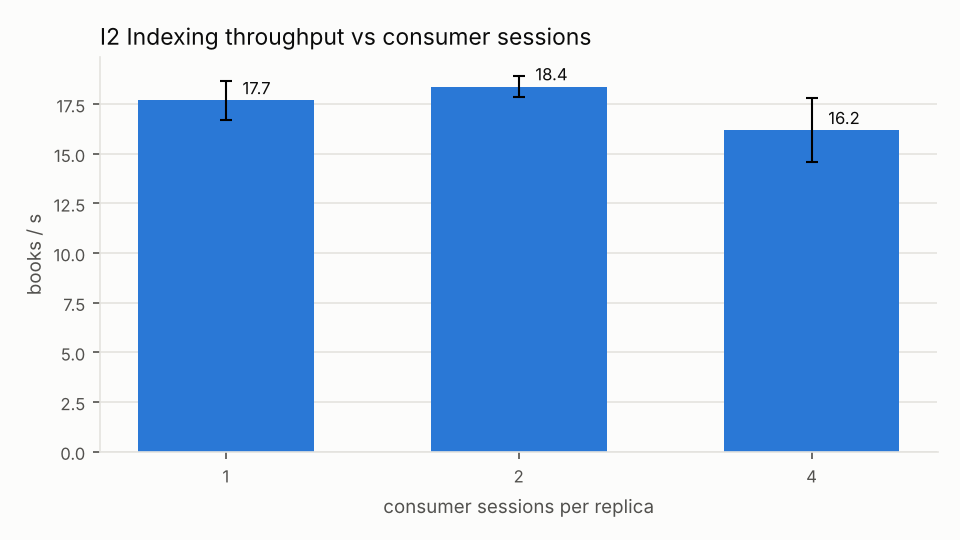
\includegraphics[width=0.75\textwidth]{i2-threads.png}
    \caption{Indexing throughput versus consumer sessions in one process.}
    \label{fig:i2}
\end{figure}

\begin{figure}[H]
    \centering
    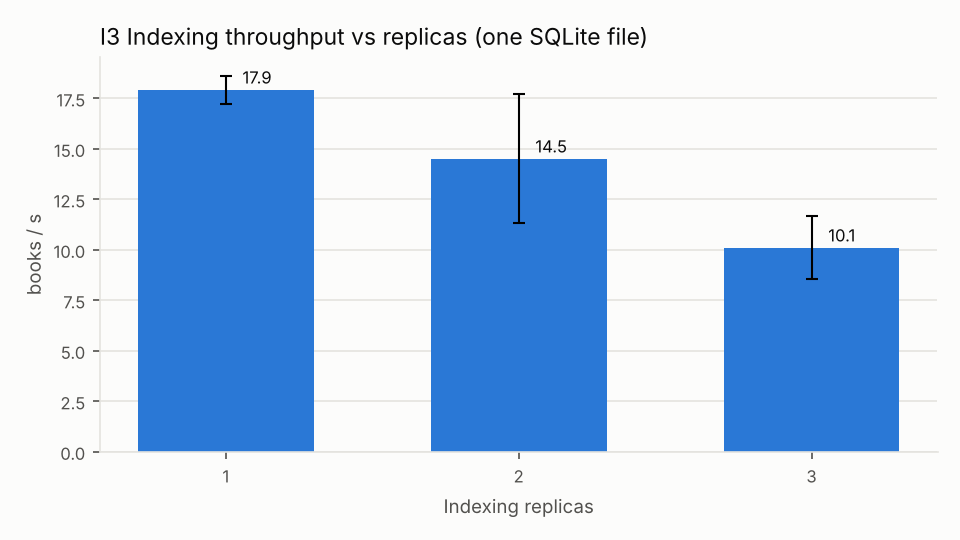
\includegraphics[width=0.75\textwidth]{i3-replicas.png}
    \caption{Indexing throughput versus Indexing replicas sharing one SQLite datamart.}
    \label{fig:i3}
\end{figure}

Batching is the factor that clearly helps. Increasing the batch from 1 to 50 messages raises
throughput by about 3.7 times because one transaction can commit many books and document-frequency
updates are aggregated. More consumer sessions do not improve throughput, and more Indexing
replicas make it worse. Three replicas achieve only about 56\% of the throughput of one replica.
The host is not CPU-saturated in this case: the replicas compete for the same SQLite writer and
spend more time waiting for access to the shared database. This identifies the single datamart
writer as the main pipeline bottleneck.

The very large request-to-completion latency in the saturated I1--I3 runs is mostly backlog time in
the \texttt{books.downloaded} queue. It should not be interpreted as the processing cost of one
book. That cost is measured separately below saturation.

\subsection{Per-Book Indexing Latency}

\begin{table}[H]
    \centering
    \caption{I4: Indexing latency below saturation, batch size 20.}
    \label{tab:i4}
    \small
    \begin{tabular}{rrrrrr}
        \toprule
        \textbf{Sent b/s} & \textbf{Indexed b/s} & \textbf{Median ms} & \textbf{Mean ms} & \textbf{p95 ms} & \textbf{Queue ms} \\
        \midrule
        2  & $2.02 \pm 0.01$ & $366 \pm 15$ & $436 \pm 44$ & $937 \pm 312$ & $2 \pm 1$ \\
        5  & $5.02 \pm 0.05$ & $337 \pm 5$  & $446 \pm 44$ & $1162 \pm 370$ & $4 \pm 3$ \\
        10 & $10.08 \pm 0.07$ & $473 \pm 32$ & $690 \pm 166$ & $1695 \pm 606$ & $27 \pm 16$ \\
        \bottomrule
    \end{tabular}
\end{table}

\begin{figure}[H]
    \centering
    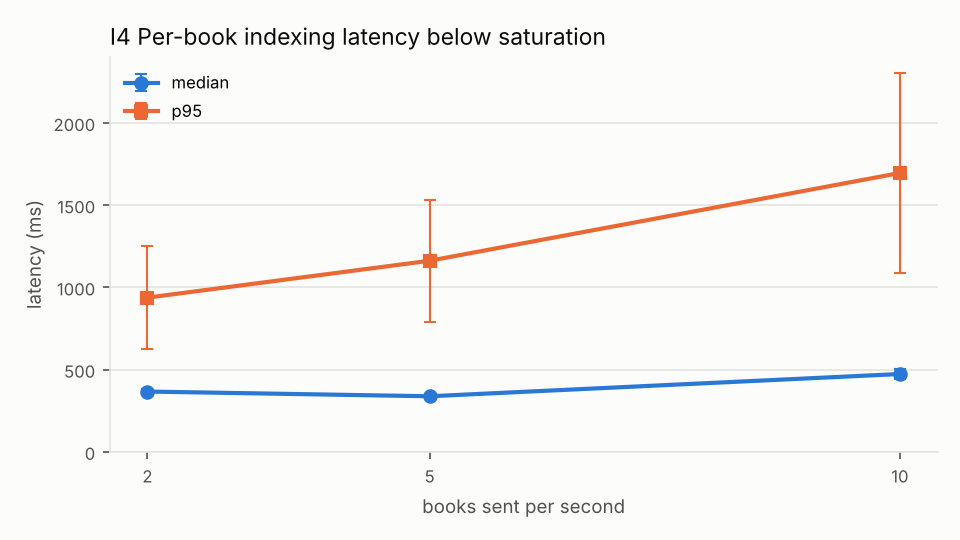
\includegraphics[width=0.78\textwidth]{i4-latency.png}
    \caption{Median, mean, and p95 per-book Indexing latency below saturation.}
    \label{fig:i4}
\end{figure}

At low and moderate input rates the median is roughly 0.35~s per book. The configured 200~ms batch
wait contributes to latency when traffic is too low to fill a batch immediately. Reducing that wait
could improve low-load latency, while larger batches are better for throughput. The longer p95 tail
varies with book size and runtime behaviour, but this experiment does not isolate one dominant
cause.

\subsection{Full Pipeline and Ingestion Replicas}

\begin{table}[H]
    \centering
    \caption{P1: full pipeline with a local Gutenberg mirror.}
    \label{tab:p1}
    \small
    \begin{tabular}{rrrrr}
        \toprule
        \textbf{Ingestion replicas} & \textbf{Ingestion b/s} & \textbf{End-to-end b/s} & \textbf{Mean latency s} & \textbf{p95 s} \\
        \midrule
        1 & $27.67 \pm 1.55$ & $16.16 \pm 0.41$ & $12.7 \pm 1.2$ & $25.3 \pm 1.1$ \\
        2 & $30.71 \pm 0.57$ & $15.46 \pm 0.09$ & $15.8 \pm 0.6$ & $31.4 \pm 0.3$ \\
        4 & $35.14 \pm 5.29$ & $14.39 \pm 0.71$ & $19.5 \pm 0.8$ & $39.5 \pm 1.1$ \\
        \bottomrule
    \end{tabular}
\end{table}

\begin{figure}[H]
    \centering
    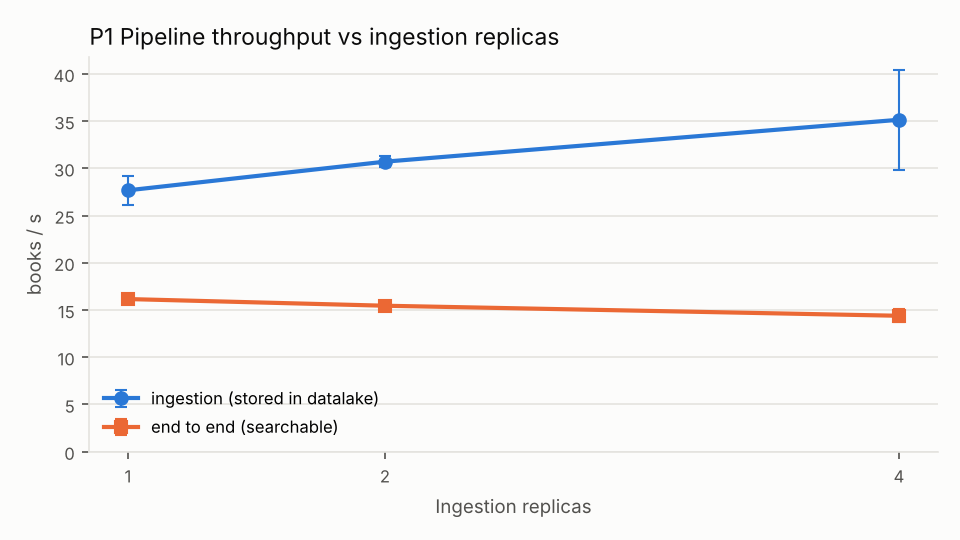
\includegraphics[width=0.78\textwidth]{p1-pipeline.png}
    \caption{Ingestion throughput and end-to-end searchable throughput as Ingestion replicas increase.}
    \label{fig:p1}
\end{figure}

Ingestion itself improves modestly with more replicas: four replicas download and split about 27\%
more books per second than one. The complete pipeline does not improve. Books become searchable at
roughly the speed at which Indexing can commit them, while the extra downloaded books wait in
\texttt{books.downloaded}. The average broker time in that queue increases from about 10 to 17
seconds. The additional Ingestion JVMs also take CPU from Indexing, so end-to-end throughput falls
slightly as more Ingestion replicas are added.

\subsection{Search and Indexing Interference}

\begin{table}[H]
    \centering
    \caption{X1: Search under load while one Indexing replica rebuilds the datamart.}
    \label{tab:x1}
    \small
    \begin{tabular}{lrrrr}
        \toprule
        & \textbf{Search q/s} & \textbf{Search p95 ms} & \textbf{Search p99 ms} & \textbf{Indexing b/s} \\
        \midrule
        Search idle & $6555 \pm 417$ & $4.96 \pm 0.35$ & $7.38 \pm 0.65$ & -- \\
        During re-index & $4696 \pm 247$ & $8.23 \pm 0.47$ & $15.16 \pm 1.09$ & $9.08 \pm 0.17$ \\
        \bottomrule
    \end{tabular}
\end{table}

\begin{figure}[H]
    \centering
    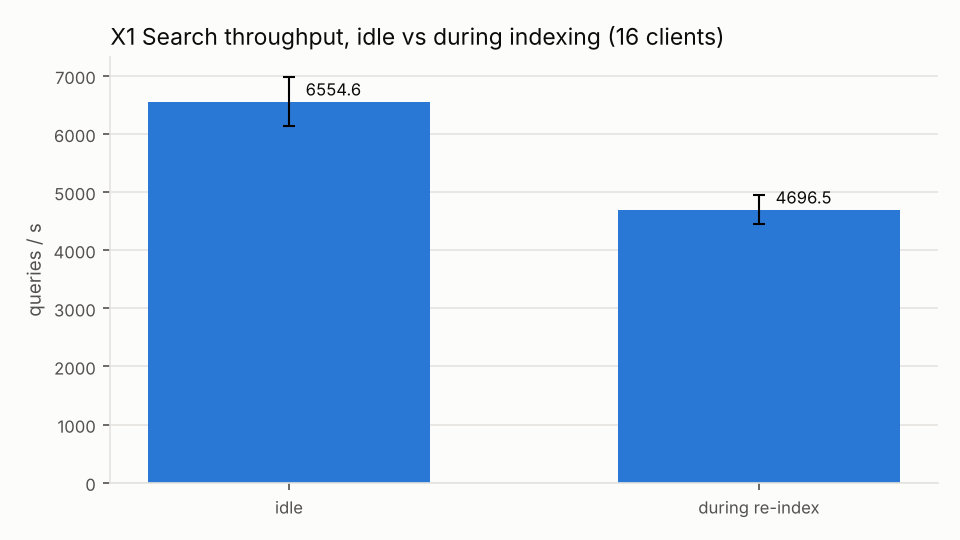
\includegraphics[width=0.70\textwidth]{x1-throughput.png}
    \caption{Search throughput with and without concurrent re-indexing.}
    \label{fig:x1-throughput}
\end{figure}

\begin{figure}[H]
    \centering
    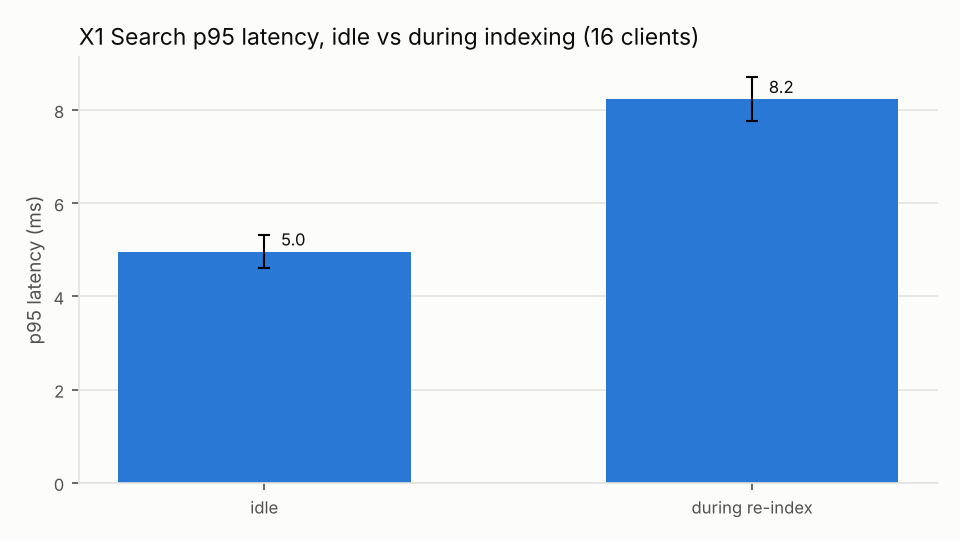
\includegraphics[width=0.70\textwidth]{x1-p95.png}
    \caption{Search p95 latency with and without concurrent re-indexing.}
    \label{fig:x1-p95}
\end{figure}

Concurrent Indexing lowers Search throughput by 28\% and increases p95 by 66\%. At the same time,
Search load reduces Indexing from about 18.4 books/s in the baseline to 9.1 books/s. WAL mode lets
readers and the writer operate concurrently, while the CPU measurements show strong competition
for the same host resources: Search uses about 5.5 logical CPUs at p90 and Indexing about 3.3.

\subsection{Coordination Cost and Resource Use}

Below saturation, broker queue time is small compared with the work itself. In I4 a message waits
about 2--27~ms in the broker while one book needs roughly 350~ms of processing latency. In the full
pipeline, \texttt{ingest.requests} waits about 1--2~ms. When the system is saturated, large queue
times are a symptom of the downstream bottleneck rather than an expensive broker operation.

\begin{table}[H]
    \centering
    \caption{Selected resource measurements, run 1 of each configuration; CPU p90 where applicable.}
    \label{tab:resources}
    \scriptsize
    \begin{tabularx}{\textwidth}{p{0.20\textwidth} p{0.20\textwidth} X p{0.20\textwidth}}
        \toprule
        \textbf{Configuration} & \textbf{Host CPU mean / p90} & \textbf{Main process CPU p90} & \textbf{Max RSS} \\
        \midrule
        S1, 32 clients & 78\% / 87\% & Search 703\% & Search 265 MiB \\
        S2, 1 replica & 72\% / 80\% & Search 646\%, nginx worker 79\% & Search 258 MiB \\
        S2, 3 replicas & 79\% / 93\% & Search 314 + 291 + 275\%, nginx 75\% & 3 $\times$ about 240 MiB \\
        I1, batch 20 & 24\% / 34\% & Indexing 380\%, broker 43\% & Indexing 1.0 GiB \\
        I3, 3 replicas & 26\% / 57\% & Indexing 301 + 266 + 291\% & 3 $\times$ about 1.0 GiB \\
        P1, 4 Ingestion replicas & 31\% / 50\% & Indexing 360\%, Ingestion about 4 $\times$ 50\% & Indexing 1.0 GiB; Ingestion about 4 $\times$ 320 MiB \\
        X1 during re-index & 37\% / 78\% & Search 547\%, Indexing 326\% & Indexing 958 MiB \\
        \bottomrule
    \end{tabularx}
\end{table}

The memory result reinforces the Indexing replica conclusion. One Indexing process can use about
1~GiB when the JVM heap and 256~MiB SQLite page cache are included. Three replicas therefore spend
about 3~GiB while still reducing throughput.

\subsection{Results Compared with Expectations}

The central expectation in the architecture document was that SQLite's single writer would limit
Indexing. The measurements confirm it more strongly than the initial design discussion suggested.
Batching improves throughput substantially, but additional consumer sessions barely help and
additional Indexing replicas make the result worse. The bottleneck is therefore not a shortage of
workers; it is serialization on one shared database file.

The Ingestion result is also consistent with the architecture. Several replicas can increase the
rate at which books are prepared, but that extra capacity is not useful while Indexing is slower.
The broker makes this imbalance visible as queue growth without blocking Ingestion itself.

The Search result is less intuitive if replication is treated automatically as a performance
optimization. One Search process already uses most of the available CPU at high client
concurrency. Adding two more processes on the same cores therefore adds overhead and lowers
throughput. This is an important distinction for Stage~3: replication can scale Search only if it
also adds physical CPU capacity, which requires separate machines or nodes.

Finally, the event broker is not the observed bottleneck. At non-saturated rates its queue delay is
a small fraction of one book's processing time, and its CPU use is about half of one logical CPU at
the measured Indexing rate. At saturation, long queue times indicate that work is waiting for
Indexing rather than that ActiveMQ is slow.

\subsection{Threats to Validity}
\label{sec:threats}

All integration measurements were collected on one laptop under WSL~2. Replicas therefore share
the same physical CPU, memory, and disk. This is the intended Stage~2 environment, but it means the
replication results cannot be generalized to a cluster where every replica has independent
hardware. In particular, the conclusion that Search replicas reduce throughput applies to this
single-host experiment, not to multi-node Search.

The benchmark client also runs on the same machine as the services. Its CPU consumption is included
in host load and can reduce the capacity available to the system being measured. CPU frequency and
thermal behaviour of the hybrid laptop processor add run-to-run variability. Every configuration
is repeated three times, but three repetitions are still a modest sample.

The local Project Gutenberg mirror removes WAN latency and server rate limiting. This is necessary
for a reproducible Ingestion experiment, but the measured Ingestion throughput describes local
CPU, parsing, and disk work rather than real Internet download speed.

The resource monitor reads Linux \texttt{/proc}. Under WSL it does not include all Windows host
activity, so the CPU and memory tables describe the Linux environment visible to the processes.
The load client itself is not shown as a separate row in the summary table even though its CPU use
is part of the host figures.

Some causes remain grouped together. The long I4 p95 tail may come from large books, garbage
collection, or SQLite checkpoints; the benchmark does not separate them. Likewise, WAL growth was
not measured independently during the Search/Indexing interference experiment. The gateway was
measured with one nginx worker, so no conclusion is made about a different gateway configuration.

% ---------------------------------------------------------------------------
\section{Conclusions and Future Improvements}
% ---------------------------------------------------------------------------
Stage~2 transforms the Stage~1 storage layer into a service-oriented search system while
preserving the same data semantics. Ingestion, Indexing, Search, the Feeder, and the broker are
independent processes, and the complete system can run with several replicas on one machine. The
shared contracts and Stage~1 oracles make it possible to add this concurrency without changing the
meaning of the tokenizer, metadata, or positional index.

The event-driven design works as intended for failure handling. Transacted acknowledgements,
persistent broker messages, idempotent consumers, atomic datalake writes, and SQLite transactions
allow work to be repeated safely. Functional tests show that the full pipeline completes after an
Indexing replica is killed, and the final combined API/event validation passes all 32 checks.

The performance results identify one clear limit. \textbf{Indexing is the bottleneck of the current
pipeline, and the bottleneck inside Indexing is the single SQLite writer.} Batching improves
throughput from about 6 to 22 books/s, but more Indexing replicas reduce it. Ingestion can prepare
books faster than Indexing can publish them, so extra Ingestion replicas only build a longer queue.
Search reaches several thousand queries per second, but on one host additional Search replicas do
not create new compute capacity and therefore do not improve throughput.

The Stage~2 results also show that replication has two different purposes. On one machine it gives
fault tolerance: a remaining replica can continue after another process dies. It does not
necessarily give performance. Performance scaling requires removing the shared resource that
serializes the work or adding hardware resources that replicas can actually use independently.

\subsection{Stage 3 Plan}

Stage~3 should preserve the logical pipeline and contracts but remove assumptions that are valid
only because all processes currently share one host.

\begin{table}[H]
    \centering
    \caption{Single-machine assumptions that must change in Stage~3.}
    \label{tab:stage3}
    \small
    \begin{tabularx}{\textwidth}{p{0.24\textwidth} p{0.31\textwidth} X}
        \toprule
        \textbf{Stage~2 assumption} & \textbf{Why it works now} & \textbf{Stage~3 direction} \\
        \midrule
        \texttt{localhost} service addresses & Every process runs inside one machine. & Real node addresses plus service discovery or explicit deployment configuration. \\
        Shared local datalake & Indexing can open files written by any Ingestion replica. & Shared/distributed storage, or transfer/ownership rules that make book data reachable across nodes. \\
        OS file locks & All Ingestion replicas share one kernel and filesystem. & Distributed ownership/partitioning or another cross-node coordination mechanism. \\
        One SQLite datamart file & One host can share one WAL database between writer and readers. & Partitioned index or database service that supports parallel writers and remote readers. \\
        Embedded single broker & One local broker is sufficient for Stage~2. & Network-reachable broker deployment with failure and unavailable-node handling. \\
        One nginx gateway & All Search replicas are local upstreams. & Gateway/load balancer that routes to Search replicas on different nodes and handles unavailable nodes. \\
        Local process manager & PIDs and \texttt{/proc} describe every component. & Cross-machine deployment, health checks, and monitoring with node identity. \\
        \bottomrule
    \end{tabularx}
\end{table}

Task distribution should also become explicit at cluster level. The current ActiveMQ queues already
provide competing-consumer distribution for Ingestion and Indexing, so their logical interface can
remain similar, but the storage behind them cannot rely on one local directory. Search is the
simpler case: replicas are read-only, so placing them on separate machines would directly add CPU
capacity once they can access a suitable distributed or replicated index.

Unavailable nodes must be treated as a normal operating condition rather than as a special test.
The Stage~2 event rules already cover redelivery after a consumer disappears; Stage~3 should extend
that idea to node discovery, storage access, gateway routing, and broker availability. The main
architectural change is therefore not the sequence of the search pipeline. It is the removal of
single-host shared state -- especially the local datalake, the SQLite single file, and the embedded
broker -- that currently prevents the measured replicas from becoming true distributed capacity.

\end{document}
